\section{Objectdetectie in sonarafbeeldingen}

\subsection{Definitie en gebruik op sonarafbeeldingen}

Objectdetectie is een tak binnen het domein van computer vision dat gericht is op het identificeren en lokaliseren van objecten binnen beelddata (zoals foto's en video's). Dit wordt gebruikt in verschillende domeinen, zoals beveiligingssystemen (bv. om inbrekers te detecteren) of de medische wereld (bv. om tumoren op te sporen). Door de jaren heen is objectdetectie aanzienlijk geëvolueerd dankzij de vooruitgang in deep learning en de grote beschikbaarheid van datasets met beeldmateriaal. \autocite{He_2016} \\

Objectdetectie combineert twee belangrijke zaken in computer vision: objectlokalisatie en objectclassificatie. Objectlokalisatie bepaalt de positie van objecten, meestal in de vorm van \glspl{bounding_box} \autocite{Tompson_2015}, terwijl objectclassificatie bepaalt tot welke categorie een gedetecteerd object behoort. Samen geeft dit de mogelijkheid tot het herkennen van verschillende soorten objecten op één foto. \\

Objectdetectie heeft vele toepassingen, ook in domeinen die misschien niet zo voor de hand liggend zijn. Één van deze specialisaties binnen de -- algemene -- objectdetectie is objectdetectie op sonardata. Dit domein is over de laatste jaren erg gegroeid, vooral onder invloed van buitenlandse dreigingen. Zo wordt sonarobjectdetectie gebruikt voor het opsporen van mijnen in zee om ze later onschadelijk te kunnen maken. Naast detectie van mijnen wordt   de techniek ook gebruikt voor verschillende soorten onderzoeken, zoals archeologisch en maritiem onderzoek. Bij deze verschillende toepassingen wordt natuurlijk telkens een kleine variatie op deze techniek gebruikt om telkens andere dingen op te sporen. \autocite{Wang_2024} \\

Traditioneel worden supervised-learning methoden gebruikt voor objectdetectie. Voorbeelden van populaire architecturen binnen dit domein zijn onder andere Faster \gls{rcnn}, \gls{yolo} en \gls{ssd}. \autocite{Redmon_2016} Omdat dit supervised-learning modellen zijn, presteren  ze uitstekend bij voldoende gelabelde data. De annotatiekosten en tijdsinvestering vormen echter een grote belemmering, vooral bij complexe datasets zoals sonar. Sonardata vereist namelijk gespecialiseerde kennis voor het labelen, wat de annotatie nog uitdagender maakt. \autocite{Long_2015} \\

Deze supervised objectdetectietechnieken vallen onder te verdelen in grofweg twee grote categorieën. Enerzijds zijn er de zogenaamde \emph{single-shot detectors}, anderzijds heb je de \emph{two-stage detectors}. Deze categorieën zijn gebaseerd op hoeveel keer de afbeelding door het netwerk gaat. Bij single-shot detectors gaat de afbeelding slechts één keer door het netwerk, bij two-stage detectors -- logischerwijs -- twee keer. \autocite{Carranza_Garcia_2020} \\

Één van de eerste succesvolle toepassingen van deep learning binnen het domein van objectdetectie gebeurde in een bekend artikel van \textcite{Girshick_2013}. In dit artikel stelden de auteurs de \gls{rcnn}-architectuur voor. Deze veelbelovende architectuur behaalde een \gls{map} van 30\% meer dan de vorige topscore op een bekende publieke dataset (\acrshort{voc} 2012).

\subsubsection{Single-shot objectdetectie}

Zoals hierboven vermeld, is een single-shot detector een model waarbij de afbeelding slechts één keer door het netwerk gaat. Dit gebeurd door een \gls{cnn} te gebruiken dat zowel objectlocaties als bijbehorende classificaties voorspelt in één enkele \emph{pass}. Het voordeel van dit soort architectuur is dat ze zeer resource-efficiënt is, aangezien elke afbeelding slechts één keer behandeld wordt. Omwille van de efficiëntie, is deze architectuur dus uitermate geschikt voor real-time toepassingen zoals autonome voertuigen en bewakingssystemen. Een nadeel is echter dat het model niet altijd even precies is, aangezien het zowel locaties als klassen in één pass moet voorspellen. Vooral bij het detecteren van kleine objecten geeft dit een probleem. Om dit -- toch gedeeltelijk -- op te lossen, wordt soms gebruik gemaakt van meerdere schaalniveaus om objecten van verschillende groottes te detecteren, wat bijdraagt aan de robuustheid en precisie. \autocite{Carranza_Garcia_2020} \\

Zowel \gls{yolo} als \gls{ssd} zijn single-shot detectors. Deze architecturen worden verder besproken in latere secties hieronder.

\subsubsection{Two-stage objectdetectie}

Zoals de naam doet vermoeden, is two-stage objectdetectie een type objectdetectie waarbij de afbeelding twee keer door het netwerk gaat. Het resultaat is nog steeds een voorspelling van locaties en klassen, maar in plaats van in één keer -- zoals bij single-shot objectdetectie -- gebeurt de voorspelling nu in twee afzonderlijke stappen. Het resultaat van de eerste \emph{pass} is een set van \emph{proposals} -- voorstellen -- en mogelijke locaties van objecten. Daarna zorgt de tweede \emph{pass} voor een verfijning van deze voorstellen. Dit zorgt dan ook voor de uiteindelijke voorspellingen. Het voordeel van dit type objectdetectie is dat het veel preciezer is dan single-shot objectdetectie, aangezien de afbeelding twee keer geanalyseerd wordt. Het nadeel is dat deze approach veel resource-intensiever is. Het is dus zaak om een afweging te maken tussen de precisie van de voorspellingen en het verbruik van resources. \autocite{Carranza_Garcia_2020} \\

Over het algemeen wordt voor real-time applicaties single-shot objectdetectie gebruikt en voor cases waar de voorspellingen heel accuraat moeten zijn, wordt two-stage objectdetectie gebruikt. Een voorbeeld van een two-stage detector is de \gls{rcnn}-architectuur van \textcite{Girshick_2013}. Ook alle latere architecturen die hierop gebaseerd zijn, zijn two-stage detectors. Voorbeelden daarvan zijn Fast \gls{rcnn}, Faster \gls{rcnn} en Mask \gls{rcnn}. \autocite{Ren_2015}

\subsection{Meten van performantie binnen objectdetectie}

Gedurende dit onderzoek zal er gewerkt worden met verschillende soorten modellen en architecturen met elk hun sterktes en hun zwaktes. Het is de bedoeling dat al deze modellen vergeleken kunnen worden met elkaar om zo het best presterende model of de best presterende modellen te kunnen selecteren. Om dit te doen zijn er standaard metrieken nodig. Deze kunnen later (tijdens de trainingsfase) dan ook dienen als \gls{loss_functie}. Er zijn enorm veel verschillende metrieken om de performantie van objectdetectiemodellen te meten, maar twee van de bekendste en meest gebruikte zijn \gls{iou} en \gls{map}.

\subsubsection{Intersection over Union (IoU)}

\gls{iou} is een heel bekende metriek om de accuraatheid van de lokalisatie binnen objectdetectiemodellen te berekenen. Om de \gls{iou} te berekenen wordt gebruikt gemaakt van de echte \gls{bounding_box} en de voorspelde \gls{bounding_box}. Eerst wordt de overlappende oppervlakte (de doorsnede of \emph{intersection} in het Engels) van de twee \glspl{bounding_box} berekend. Daarna wordt de totale oppervlakte (de unie of \emph{union} in het engels) van de twee \glspl{bounding_box} berekend. \\

Door de doorsnede te delen door de unie krijgt men een verhouding van de overlappende oppervlakte tot de totale oppervlakte. Dit geeft een goede indicatie van hoe dicht de voorspelde \gls{bounding_box} bij de echte \gls{bounding_box} ligt. Een lagere \gls{iou}-score duidt op een betere prestatie, aangezien de voorspelde \gls{bounding_box} niet dan weinig afwijkt van de echte \gls{bounding_box}. \autocite{Rezatofighi_2019}

\begin{figure}[H]
    \centering
    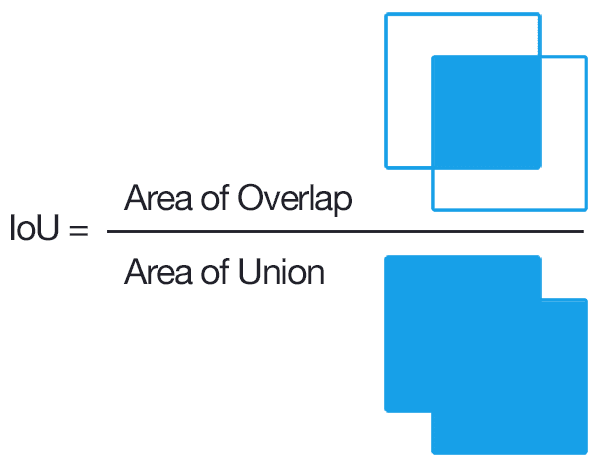
\includegraphics[width=0.5\textwidth]{iou_equation.png}
    \caption[Voorstelling van IoU.]{\label{fig:iou_equation}Formule en visuele voorstelling van de \acrfull{iou}. \autocite{Rosebrock_2016}}
\end{figure}

\subsubsection{mean Average Precision (mAP)}

Een andere -- zeer bekende -- metriek is de \acrfull{map}. Ze beoordeelt de nauwkeurigheid van een model op basis van zowel \gls{precision} als \gls{recall}. Het wordt berekend door de gemiddelde precisie (of \emph{average precision}, AP) over alle klassen en \gls{iou} drempels te bepalen. AP wordt verkregen door de oppervlakte onder de precisie-recallcurve van een specifieke klasse te berekenen door hem te integreren, en \gls{map} is vervolgens het gemiddelde van deze waarden over alle klassen. Een hogere mAP-score duidt op betere prestaties van een objectdetectiemodel, omdat het aangeeft hoe goed het model objecten correct detecteert en classificeert. \autocite{Wang_2022}

\subsection{Typische uitdagingen bij sonarobjectdetectie}

Objectdetectie op sonarbeelden die gemaakt zijn onderwater wordt geconfronteerd met verschillende uitdagingen die de nauwkeurigheid en betrouwbaarheid van detecties beïnvloeden.

Ruis is een van de voornaamste obstakels bij sonarobjectdetectie. Onderwateromgevingen zijn inherent lawaaierig door factoren zoals luchtbellen, \glspl{thermocline} en biologische organismen, wat leidt tot significante ruis in sonarbeelden. Deze ruis bemoeilijkt het onderscheiden van echte objecten van artefacten typisch aan sonarbeelden, waardoor de betrouwbaarheid van de detecties afneemt. \autocite{Aubard_2024_Datasets} \\

Een andere uitdaging is de lage resolutie van sonarbeelden. In vergelijking met optische sensoren leveren sonars vaak beelden met beperkte detailweergave, wat de identificatie en classificatie van objecten moeilijker maakt. Deze beperking is vooral problematisch bij het detecteren van kleine of complexe objecten, waar detailniveau essentieel is voor nauwkeurige herkenning. \autocite{Lee_2018} \\

Daarnaast zorgen variërende omstandigheden in de onderwateromgeving voor extra complicaties. Factoren zoals veranderende waterdieptes, temperatuurverschillen, stromingen en de aanwezigheid van zwevende deeltjes kunnen de prestaties van sonarsystemen beïnvloeden. Deze dynamische omstandigheden kunnen leiden tot variaties in signaalsterkte en -kwaliteit, wat de consistentie van objectdetectie bemoeilijkt. \autocite{Valdenegro_Toro_2019} \\

Het overwinnen van deze uitdagingen vereist geavanceerde signaalverwerkingstechnieken en robuuste algoritmen die kunnen omgaan met ruis, lage resolutie en variabele omgevingsfactoren. Door voortdurende technologische innovaties en onderzoek kunnen de prestaties van sonarobjectdetectiesystemen worden verbeterd, wat leidt tot betrouwbaardere toepassingen in onderwateromgevingen.

\subsection{Overzicht van bestaande technieken}

Grofweg zijn er twee stromingen van objectdetectie op sonarafbeeldingen. Enerzijds zijn er de klassieke methoden en anderzijds zijn er de moderne deep learning-technieken. De klassieke methoden werden vooral gebruikt in een tijd waar grote, complexe neurale netwerken trainen onmogelijk was bij gebrek aan voldoende computerkracht, maar worden de dag van vandaag nog altijd gebruikt als pre-processing technieken voor de datasets waarmee de moderne neurale netwerken getraind worden. Deze klassieke methoden berusten enkel op statistische technieken om zo objecten in afbeeldingen te proberen detecteren. Specifiek zijn deze vooral gericht op het verbeteren van beeldkwaliteit en het onderscheiden van objecten van de achtergrond.

\subsubsection{Filtertechnieken}

Een voorbeeld van een klassieke methode zijn filtertechnieken. Deze worden toegepast om ruis in sonarafbeeldingen te verminderen en de beeldkwaliteit te verbeteren. Er bestaan immens veel verschillende soorten filters die elk geoptimaliseerd voor een specifiek doel. Een veelgebruikte filtermethode is het gebruik van adaptieve filters die zich aanpassen aan de lokale kenmerken van het beeld. Een voorbeeld hiervan is te vinden in een artikel van \textcite{Aridgides_1995}. Merk op dat dit inderdaad een relatief oude publicatie is, wat aantoont dat deze technieken al gebruikt werden toen deep learning-gebaseerde objectdetectie niet mogelijk was. \\

In dit artikel introduceren de auteurs een adaptieve filtertechniek die ontwikkeld is om mijnachtige doelen te onderscheiden van achtergrondruis in sonarbeelden. De filter onderdrukt achtergrondruis terwijl het de target behoudt. De procedure omvat vier stappen: het berekenen van een genormaliseerde gemiddelde target, het bepalen van de covariantiematrix van de achtergrondruis, het oplossen van normale vergelijkingen om een adaptief filter te verkrijgen en het toepassen van een 2D-filter op de gegevens. Dit algoritme bewijst dat, hoewel er geen gebruik gemaakt wordt van deep-learningtechnieken, ze toch complex kan zijn. De techniek heeft in verschillende testen prestaties geleverd die vergelijkbaar zijn met die van een ervaren sonaroperator. \\

Adaptieve filters worden ook vandaag de dag nog gebruikt, wat aangetoond wordt door een paper van \textcite{Lourey_2017}. Hierin wordt ook een filtertechniek beschreven die toegepast kan worden op \gls{cas} om interferentie van de directe transmissie en de echo van de target van elkaar te onderscheiden. Deze methode kan als effectieve pre-processing techniek gebruikt worden voor trainingsdata.

\subsubsection{Thresholding}

Naast filtering bestaan er nog andere klassieke methoden. Een \emph{straightforward}-aanpak is een simpele \emph{threshold}. Thresholding is een techniek waarbij pixelwaarden worden vergeleken met een bepaalde drempelwaarde om objecten van de achtergrond te scheiden. Een klassieke benadering is de Otsu-methode, die de interklassevariantie minimaliseert om een optimale drempelwaarde te bepalen. Deze methode wordt beschreven in een artikel van \textcite{Otsu_1979}.

\begin{figure}[H]
    \centering
    \begin{subfigure}{.5\textwidth}
        \centering
        \captionsetup{justification=centering}
        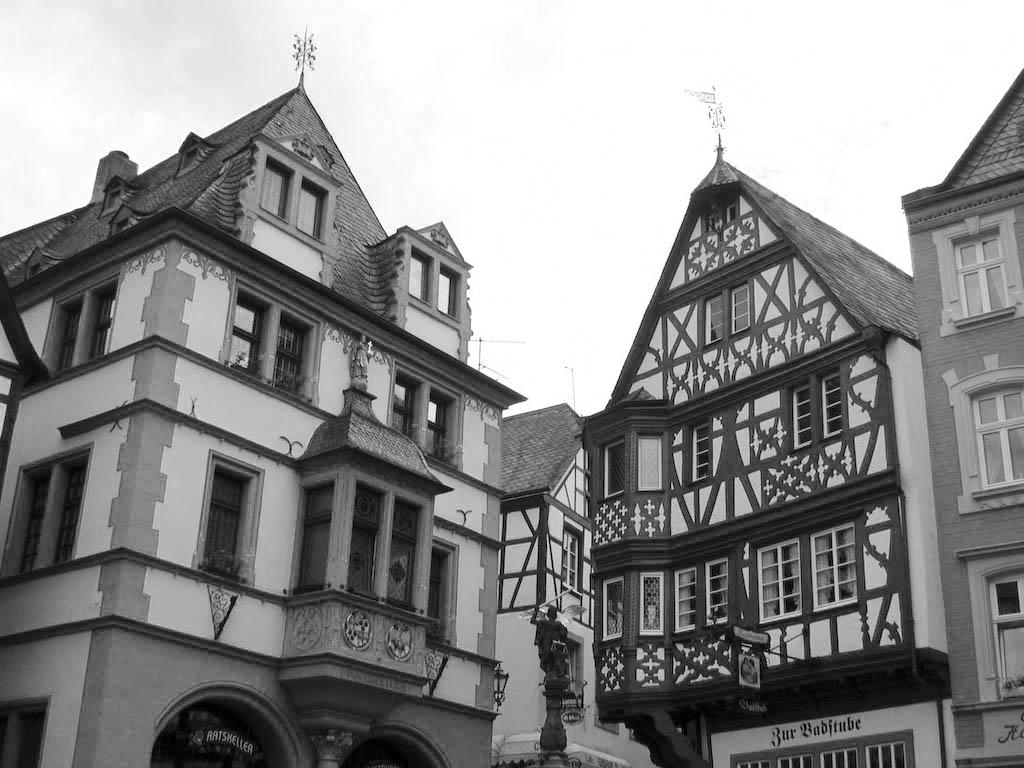
\includegraphics[width=0.9\linewidth]{img_pre_otsu.jpg}
        \caption[Afbeelding voor Otsu's thresholding]{Afbeelding voor Otsu's thresholding. \autocite{http//www.freephotos.lu/_2010}}
        \label{fig:img_pre_otsu}
    \end{subfigure}%
    \begin{subfigure}{.5\textwidth}
        \centering
        \captionsetup{justification=centering}
        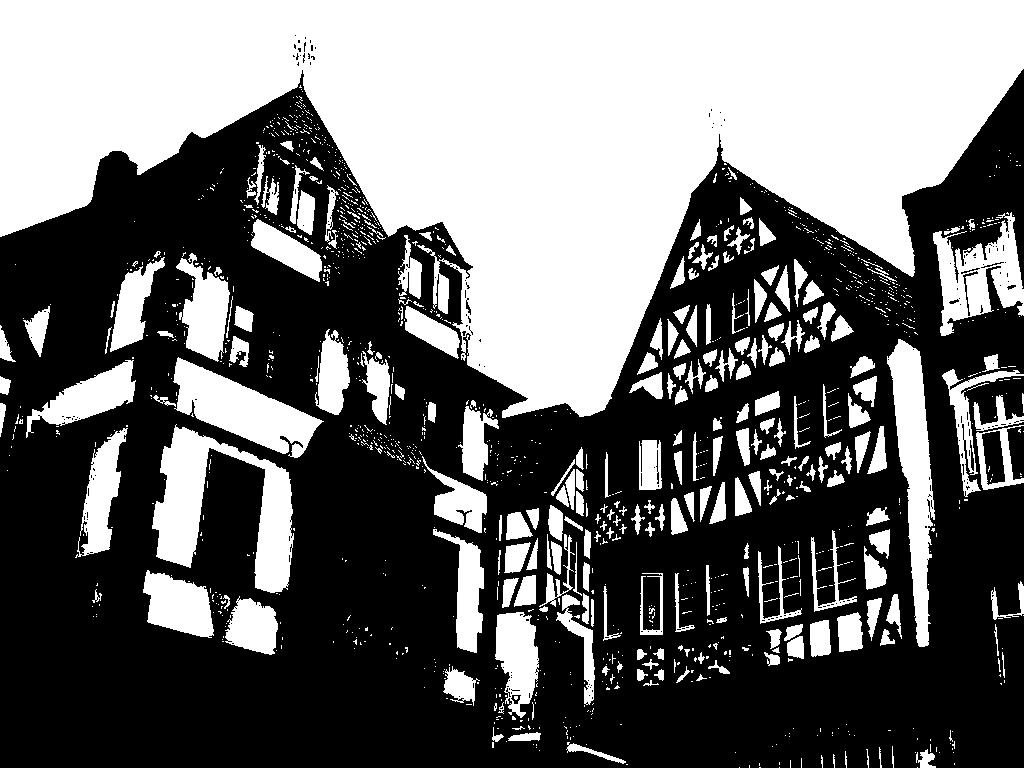
\includegraphics[width=0.9\linewidth]{img_post_otsu.jpg}
        \caption[Afbeelding na Otsu's thresholding]{Afbeelding na Otsu's thresholding. \autocite{Pikez33_2010}}
        \label{fig:img_post_otsu}
    \end{subfigure}
    \caption[Afbeelding voor en na Otsu's thresholding]{Afbeelding voor en na Otsu's thresholding}
    \label{fig:imgs_otsu}
\end{figure}

Hoewel deze techniek oorspronkelijk is ontwikkeld voor visuele beelden, is deze ook toegepast op sonarafbeeldingen, zoals besproken in verschillende artikels, waaronder dat van \textcite{Yuan_2016} en dat van \textcite{Dimitrova_Grekow_2017}. Ondanks zijn simpliciteit kan deze techniek aanzienlijke verbeteringen teweegbrengen. Dit wordt onder andere aangehaald in een paper van \textcite{Komari_Alaie_2018}. Deze paper onderzoekt objectdetectie met passieve sonar in de Perzische Golf. Aangezien deze binnenzee ondiep is, is er sprake van een hoge hoeveelheid fouten tijdens de detectie. Een bepaald soort adaptieve thresholding-techniek kon de \gls{precision} van hun objectdetectiemodel met 24\% verbeteren.

\subsubsection{Edge detection}

Edge detection is een andere klassieke techniek die wordt gebruikt om de contouren van objecten in sonarafbeeldingen te identificeren. \autocite{Torre_1986} Een bekende methode is de Canny edge detector, die randen detecteert door het maximaliseren van de gradiëntgrootte. Deze techniek komt als beste uit de vergelijkende studie van \textcite{Awalludin_2022}. \\

De Canny edge detector werkt in meerdere stappen om nauwkeurige en robuuste contourdetectie te realiseren. De eerste stap is Gaussian blurring, waarbij het beeld wordt vervaagd om ruis te verminderen en kleine details die geen significante randen vormen te onderdrukken. Vervolgens wordt de gradiënt van het beeld berekend met behulp van Sobel-operatoren in zowel de horizontale als verticale richting, waardoor de randen worden geaccentueerd. Daarna wordt non-maximum suppression toegepast, waarbij alleen de sterkste randen worden behouden en omliggende pixels met lagere gradiëntwaarden worden onderdrukt. De laatste stap is hysteresis thresholding, waarbij twee drempelwaarden worden gebruikt: pixels met een gradiëntsterkte boven de hoge drempel worden als randen geclassificeerd, terwijl pixels onder de lage drempel worden genegeerd. Pixels met tussenliggende waarden worden alleen als rand beschouwd als ze verbonden zijn met een sterke randpixel. Dankzij deze gefaseerde aanpak is de Canny-methode effectief in het detecteren van duidelijke randen, zelfs in ruisgevoelige omgevingen zoals sonarafbeeldingen. \autocite{Ding_2001} \\

Ook edge detection wordt vandaag de dag nog gebruikt om een grote bijdrage te leveren aan bijvoorbeeld segmentatiemodellen. Het onderzoek van \textcite{Priyadharsini_2019} gebruikt gespecialiseerde edge detection als pre-processing voor de data naar een objectdetectiemodel gaat. \\

Deze klassieke technieken vormen de basis voor objectdetectie in sonarafbeeldingen en hebben bijgedragen aan de ontwikkeling van meer geavanceerde methoden. Ze blijven relevant, vooral in situaties waarin resources beperkt zijn of wanneer eenvoud en interpretatie van het model belangrijk zijn. Ze worden tot op de dag van vandaag gebruikt als pre-processing stap, bijvoorbeeld. Doordat computerkracht steeds goedkoper en meer beschikbaar werd, wordt tegenwoordig vaak gekozen voor deep learning-oplossingen voor deze problemen. Er zijn gespecialiseerde architecturen ontwikkeld om objectdetectie uit te voeren. Hieronder worden er enkele besproken.

\subsubsection{YOLO}

\acrfull{yolo} is een deep learning-gebaseerde architectuur voor objectdetectie dat bekend staat om zijn snelheid en efficiëntie. Het werd voor het eerst geïntroduceerd in een artikel van \textcite{Redmon_2016} en is sindsdien één van de populairste algoritmes in computervisie. In tegenstelling tot traditionele detectiemethoden, waar objecten in meerdere stappen geanalyseerd worden, verwerkt YOLO een afbeelding in één enkele \emph{pass} van het neurale netwerk. Dit zorgt ervoor dat real-time objectdetectie mogelijk is, waardoor het bijzonder geschikt is voor toepassingen zoals autonome voertuigen, videobewaking en \gls{ar}.

\begin{figure}[H]
    \centering
    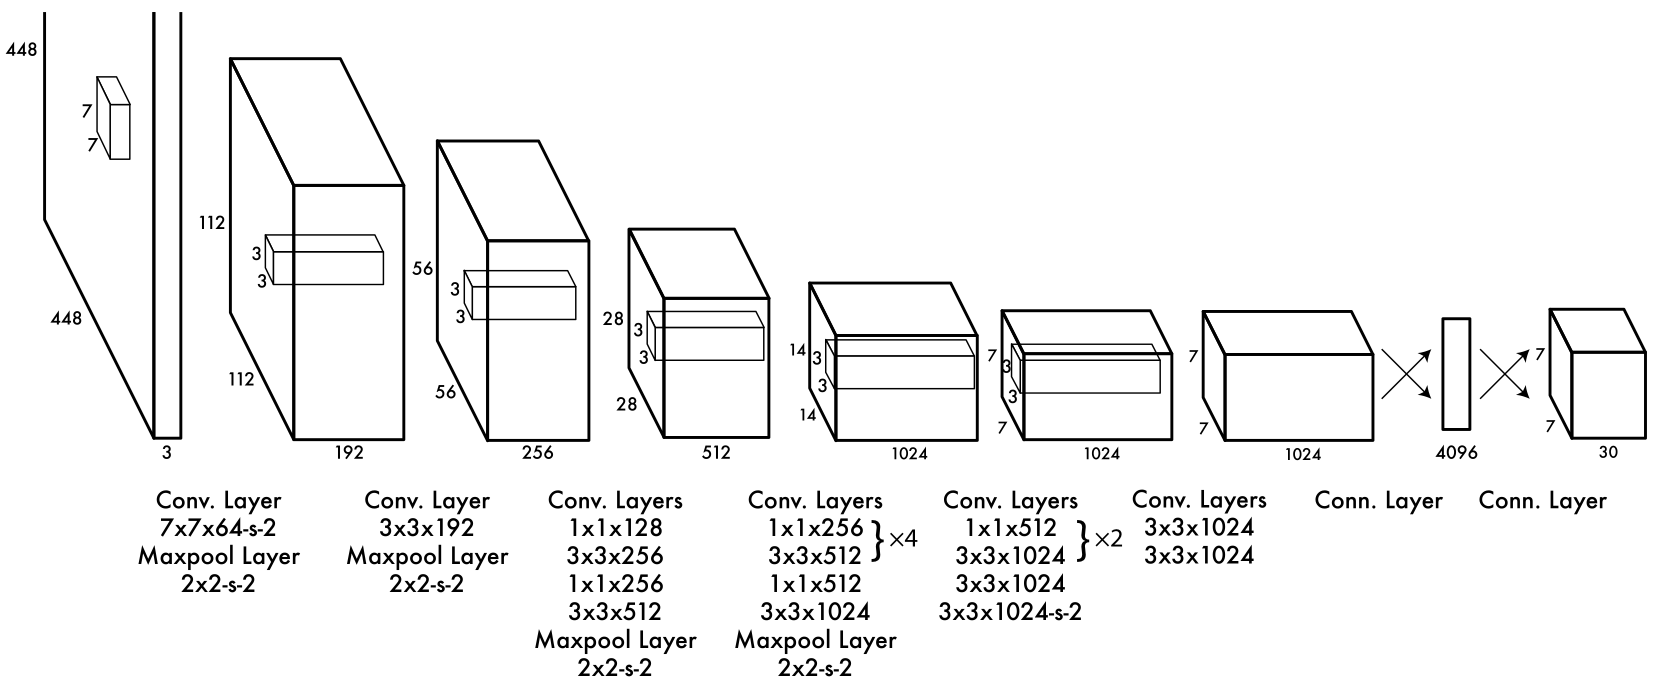
\includegraphics[width=\textwidth]{yolo_architecture.png}
    \caption[Originele YOLO-architectuur.]{\label{fig:yolo_architecture}Schematische voorstelling van de originele YOLO-architectuur. \autocite{Redmon_2016}}
\end{figure}

\gls{yolo} gebruikt een \gls{cnn} om objecten direct te lokaliseren en classificeren, wat bijdraagt aan de hoge nauwkeurigheid en snelheid van het model. De eerste versie van \gls{yolo} gebruikt ImageNet om de eerste 20 convolutionele lagen te pre-trainen. Het model wordt daarna omgezet om detectie uit te voeren, aangezien de combinatie van convolutionele lagen en fully-connected-lagen de performantie verhoogt. \autocite{Redmon_2016} De interne werking van \gls{yolo} kan opgesplitst worden in verschillende fasen. \\

Eerst en vooral wordt de invoerafbeelding opgesplitst in een $S \times S$ raster (bv. $7 \times 7$). Elke cel van dat raster is daarna verantwoordelijk voor het detecteren van objecten waarvan het midden zich in dat vak bevindt. Voor elke cel voorspelt \gls{yolo} meerdere \glspl{bounding_box}. Zo'n voorspelling van een \gls{bounding_box} bevat telkens 5 parameters (cf. \ref{fig:bounding_box}): 

\begin{itemize}
    \item $x$ en $y$: de gecentreerde coördinaten van het object binnen de cel in het raster.
    \item $w$ en $h$: de breedte en hoogte van het object, genormaliseerd ten opzichte van de afbeelding.
    \item De \gls{confidence_score}: de waarschijnlijkheid dat er daadwerkelijk een object in de box zit.
\end{itemize}

Naast het voorspellen van de \glspl{bounding_box} voorspelt het model ook de klasse van het object (bv. auto, hond, persoon, \dots) en de \gls{confidence_score} van deze classificatie. Echter zijn er vaak meerdere \glspl{bounding_box} die hetzelfde object detecteren. Daarom gebruikt \gls{yolo} \gls{nms} om overbodige detecties te verwijderen. Ten slotte genereert \gls{yolo} een lijst met gedetecteerde objecten, hun locaties en de waarschijnlijkheid van hun klassen. \autocite{Diwan_2022} \\

\gls{yolo} is sneller dan traditionele methoden zoals Faster R-CNN omdat het objectdetectie beschouwt als een enkel regressieprobleem. Dit betekent dat het model direct van ruwe pixels naar detecties gaat, zonder een apart proces voor regio-voorstel en classificatie. \\

Sinds de introductie van \gls{yolo} in de paper van \textcite{Redmon_2016} heeft het model aanzienlijke verbeteringen en evoluties doorgemaakt. De oorspronkelijke versie, \gls{yolo}v1, legde de basis met een enkelvoudige doorvoer voor objectdetectie, maar had beperkingen in nauwkeurigheid, vooral bij kleine objecten. \gls{yolo}v2 (ook wel \gls{yolo}9000) werd kort na de introductie van het originele \gls{yolo}-model geïntroduceerd in een paper van \textcite{Redmon_2016_YOLOv2}. De nieuwe versie werd ontwikkeld om sneller en accurater te zijn dan het originele model. Ook kon deze versie meer verschillende klassen onderscheiden. Daarnaast werd er gebruik gemaakt van een andere \emph{backbone}, namelijk Darknet-19 (wat zelf een variant is van VGGNet). Dit zijn de belangrijkste veranderingen:

\begin{itemize}
    \item Gebruik van een nieuwe \gls{loss_functie} die beter geschikt is voor objectdetectie.
    \item Gebruik van \gls{batch_normalisatie} om accuraatheid en stabiliteit te verhogen.
    \item Trainen op zelfde afbeeldingen met een verschillende schaal, hierdoor wordt het model beter in het herkennen van kleine objecten.
    \item Gebruik van zogenaamde \emph{anchor boxes}: dit zijn vooraf gedefinieerde \glspl{bounding_box} die helpen bij het detecteren van objecten in een afbeelding. Tijdens het trainen leert het model welke van deze \emph{anchor boxes} het beste passen bij de werkelijke objecten in de afbeelding.
\end{itemize}

\gls{yolo}v3 werd geïntroduceerd in een paper van \textcite{Redmon_2018}. Het doel van deze iteratie was opnieuw het verbeteren van de accuraatheid en de snelheid. Dit deden de onderzoekers door opnieuw een andere architectuur te gebruiken als \emph{backbone}. Dit keer gebruikten ze Darknet-53 (een variant van ResNet). Daarnaast werden de \emph{anchor boxes} aangepast zodat ze verschillende vormen en maten hadden (in tegenstelling tot allemaal dezelfde vorm en maat in \gls{yolo}v2). Ook werden nog andere technieken toegepast om kleine objecten efficiënter en beter te kunnen detecteren. \\

De ontwikkeling van \gls{yolo} werd overgenomen door andere mensen, aangezien Joseph Redmond (de originele ontwikkelaar) na \gls{yolo}v3 de AI-community verliet. In een paper van \textcite{Bochkovskiy_2020} werd \gls{yolo}v4 geïntroduceerd. Hierin werd de efficiëntie verder verhoogd door verbeterde activatiefuncties en optimalisatietechnieken. \gls{yolo}v5, geïntroduceerd door Ultralytics, richtte zich op gebruiksvriendelijkheid en efficiëntere implementatie. \autocite{Jiang_2022} Nieuwere versies, zoals \gls{yolo}v7 en \gls{yolo}v8, blijven innoveren met hogere detectienauwkeurigheid, verbeterde verwerkingstijden en geavanceerdere architecturen, waardoor \gls{yolo} één van de meest gebruikte objectdetectiemodellen blijft in real-time toepassingen. \autocite{Terven_2023} \\

Ook heeft de architectuur veel potentie voor onderwaterobjectdetectie, zoals bij het opsporen van wrakken, onderzeese mijnen en mariene organismen. Dankzij de snelheid en efficiëntie van \gls{yolo} kunnen real-time detecties worden uitgevoerd, wat waardevol is voor \glspl{auv} en robots die in onbekende of gevaarlijke omgevingen opereren. Bovendien kunnen verbeterde versies van \gls{yolo}, zoals \gls{yolo}v5 en \gls{yolo}v8, met aangepaste architecturen en pre-processingtechnieken betere resultaten behalen op sonarbeelden. Door de voortdurende ontwikkeling van deep learning en sonarverwerking wordt \gls{yolo} steeds vaker ingezet voor geavanceerde onderwaterdetectie en navigatie. \autocite{Chen_2023}

\subsubsection{Faster R-CNN}

\lipsum[1]

\autocite{Ren_2015}
\autocite{Wang_2023}
\autocite{Zeng_2021}
\autocite{Yulin_2020}

\subsubsection{SSD}

\lipsum[1]

\autocite{Ma_2020}
\autocite{Kumar_2020}
\autocite{Liu_2016}
\autocite{Jiang_2020}

\subsection{Specifieke toepassingen}

\lipsum[1-3]